\documentclass[12pt]{article}
\usepackage[parfill]{parskip}
\usepackage{amsmath}
\usepackage{amssymb}
\usepackage{bm}
\usepackage{enumerate}
\usepackage{fancyvrb}
\usepackage[top=1in, bottom=1in, left=1in, right=1in]{geometry}
\usepackage{hyperref}
\hypersetup{
    colorlinks=true,
}
\usepackage{placeins}
\usepackage{tikz}
\usepackage{tikzsymbols}
\usepackage{todonotes}
\usepackage{bbm}
\usepackage{color}
\usepackage{enumitem}
\usepackage{xcolor}
\newcommand{\rmn}[1]{{\textcolor{blue}{\bf [{\sc rmn:} #1]}}}
\DeclareMathOperator*{\argmax}{arg\,max}
\usepackage{algorithmicx}
\usepackage{algorithm}
\usepackage{algpseudocode}

\usetikzlibrary{positioning,calc}
%%%%%%%%%
\usepackage[most]{tcolorbox}
\newtcolorbox[]{solution}[1][]{%
    breakable,
    enhanced,
    colback=white,
    title=Solution,
    #1
}
%%%%%%%%%%
\title{10-703 Deep Reinforcement Learning and Control\\
  Assignment 3\\
  Spring 2018
}
\date{March 26, 2018\\
  \hspace{1cm}\\
Due April 9, 2018, 11:59pm (EST)}

\begin{document}

\maketitle

\section*{Instructions}

You may work in teams of \textbf{2} on this assignment. Only one person should submit the writeup and code on Gradescope. Additionally, the same person who submitted the writeup and code to Gradescope must upload the code to Autolab.  Make sure you mark your partner as a collaborator on Gradescope (you do not need to do this in Autolab) and that both names are listed in the writeup.  Writeups should be typeset in \LaTeX and submitted as PDF. All code, including auxiliary scripts used for testing, should be submitted with a README.

Please limit your writeup to 8 pages or less (excluding the provided instructions).

We've provided some code templates (using Keras) that you can use if you wish. Abiding to the function signatures defined in these templates is not mandatory; you can write your code from scratch if you wish. You can use any deep learning package of your choice (e.g., Keras, Tensorflow, PyTorch). However, if you choose not to use Keras, then you'll need to figure out how to load the policy network architecture (\texttt{LunarLander-v2-config.json}) and the expert's weights (\texttt{LunarLander-v2-weights.h5}).

You should not need the cluster or a GPU for this assignment. The models are small enough that you can train on a laptop CPU.

It is expected that all of the work you submit is your own. Submitting a classmate's code or code which copied from online and claiming it is your own is not allowed. Anyone who does this will be violating University policy, and risks failure of the assignment, course and possibly disciplinary action taken by the university.

\section*{Introduction}

In this assignment, you will implement different RL algorithms and evaluate them on the LunarLander-v2 environment (Figure~\ref{fig:lunarlander-v2}). This environment is considered solved if the agent can achieve an average score of at least 200.

\begin{center}
\begin{figure}[h]\centering
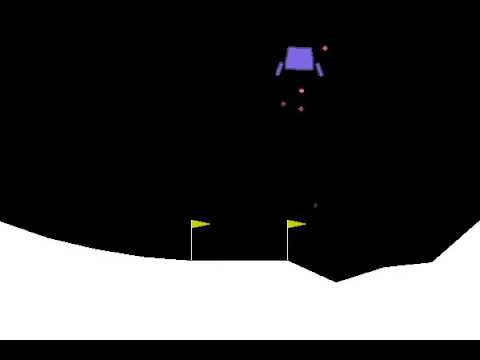
\includegraphics[width=0.4\textwidth]{lunarlander.jpg}
\caption{LunarLander-v2: \url{https://gym.openai.com/envs/LunarLander-v2/} \label{fig:lunarlander-v2}}
\end{figure}
\end{center}

\subsection*{Installation instructions (Linux)}

We've provided Python packages that you may need in \texttt{requirements.txt}. To install these packages using pip and virtualenv, run the following commands:
\begin{quote}
\begin{verbatim}
apt-get install swig
virtualenv env
source env/bin/activate
pip install -U -r requirements.txt
\end{verbatim}
\end{quote}
If your installation is successful, then you should be able to run the provided template code:
\begin{quote}
\begin{verbatim}
python imitation.py
python reinforce.py
python a2c.py
\end{verbatim}
\end{quote}

Note: You will need to install \texttt{swig} and \texttt{box2d} in order to install \texttt{gym[box2d]}, which contains the \texttt{LunarLander-v2} environment. You can install \texttt{box2d} by running
\begin{quote}
\texttt{pip install git+https://github.com/pybox2d/pybox2d}
\end{quote}
If you simply do \texttt{pip install box2d}, you may get an error because the pip package for \texttt{box2d} depends on an older version of \texttt{swig}.\footnote{\url{https://github.com/openai/gym/issues/100}} For additional installation instructions, see \url{https://github.com/openai/gym}.

\newpage
\section*{Problem 1: Imitation Learning (30 pts)}

In this section, you will implement behavior cloning using supervised imitation learning from an expert policy, and test on the LunarLander-v2 environment. Please write your code in \texttt{imitation.py}; the template code provided inside is there to give you an idea on how you can structure your code, but is not mandatory to use.

We have provided you with an expert, which you will use to generate training data that you can use with the Keras \texttt{fit} method. The expert model's network architecture is given in \texttt{LunarLander-v2-config.json} and the expert weights in \texttt{LunarLander-v2-weights.h5}. You can load the expert model using the following code snippet:
\begin{quote}
\begin{verbatim}
import keras

model_config_path = 'LunarLander-v2-config.json'
with open(model_config_path, 'r') as f:
    expert = keras.models.model_from_json(f.read())

model_weights_path = 'LunarLander-v2-weights.h5f'
expert.load_weights(model_weights_path)
\end{verbatim}
\end{quote}

Tasks and questions:
\begin{enumerate}
\item Use the provided expert model to generate training datasets consisting of 1, 10, 50, and 100 expert episodes. You will need to collect states and a one-hot encoding of the expert's selected actions.

\item Use each of the datasets to train a cloned behavior using supervised learning. For the cloned model, use the same network architecture provided in \texttt{LunarLander-v2-config.json}. When cloning the behavior, we recommend using the Keras \texttt{fit} method. You should compile the model with cross-entropy as the loss function, Adam as the optimizer, and include `accuracy' as a metric. 

For each cloned model, record the final training accuracy after training for at least 50 epochs. Training accuracy is the fraction of training datapoints where the cloned policy successfully replicates the expert policy. Make sure you include any hyperparameters in your report. 

\item Run the expert policy and each of your cloned models on \texttt{LunarLander-v2}, and record the mean/std of the total reward over 50 episodes. How does the amount of training data affect the cloned policy? How do the cloned policies' performance compare with that of the expert policy?
\end{enumerate}

\newpage
\section*{Problem 2: REINFORCE (30 pts)}

In this section, you will implement episodic REINFORCE, a policy-gradient learning algorithm. Please write your code in \texttt{reinforce.py}; the template code provided inside is there to give you an idea on how you can structure your code, but is not mandatory to use.

Policy gradient methods directly optimize the policy $\pi(A \mid S, \theta)$, which is parameterized by $\theta$. The REINFORCE algorithm proceeds as follows. We keep running episodes. After each episode ends, for each time step $t$ during that episode, we alter the parameter $\theta$ with the REINFORCE update. This update is proportional to the product of the return $G_t$ experienced from time step $t$ until the end of the episode and the gradient of $\ln \pi(A_t \mid S_t, \theta)$. See Fig.~\ref{REINFORCE} for details.

\begin{center}\begin{figure}[h]
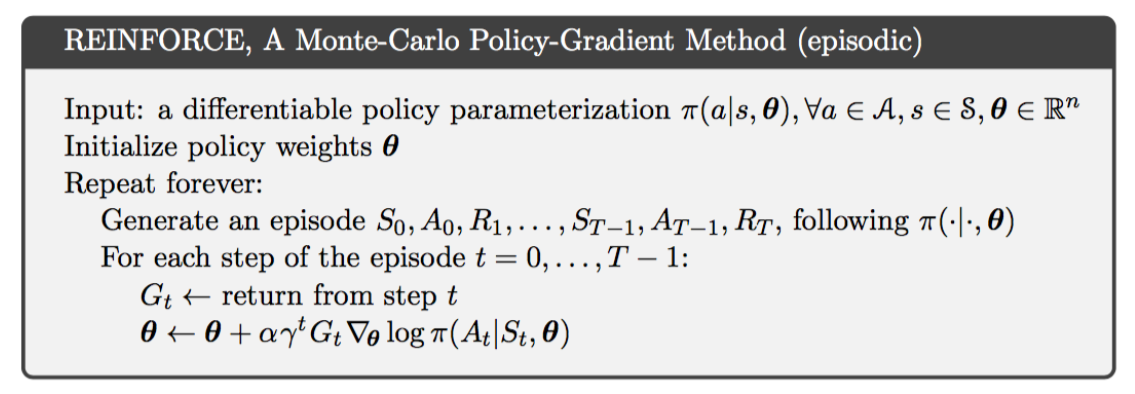
\includegraphics[width=\textwidth]{REINFORCE.png}
\caption{\label{REINFORCE} REINFORCE algorithm, covered in Sections 13.3 of Sutton \& Barto's RL book (\url{http://incompleteideas.net/book/bookdraft2018feb28.pdf\#page=287}) and in the ``Policy Gradient II'' Lecture (\url{http://www.cs.cmu.edu/~rsalakhu/10703/Lectures/Lecture\_PG2.pdf}).}
\end{figure}
\end{center}

For the policy model $\pi(A \mid S, \bf{\theta})$, use the network config provided in \\\texttt{LunarLander-v2-config.json}. It already has a softmax output so you shouldn't have to modify the config. As shown in the template code, you can load the model by doing:
\begin{quote}
\begin{verbatim}
with open('LunarLander-v2-config.json', 'r') as f:
    model = keras.models.model_from_json(f.read())
\end{verbatim}
\end{quote}
You can choose which optimizer and hyperparameters to use, so long as they work for learning on \texttt{LunarLander-v2}. We recommend using Adam as the optimizer. It will automatically adjust the learning rate based on the statistics of the gradients it's observing. Think of it like a fancier SGD with momentum. Both Tensorflow and Keras provide versions of Adam.

Downscale the rewards by a factor of 1e-2 (i.e., divide by 100) when training (but not when plotting the learning curve). When you implement A2C in the next section, this will help with the optimization since the initial weights of the Critic are far away from being able to predict a large range such as $[-200, 200]$.

To train the policy model, you need to take the gradient of the log of the policy. This is simple to do with Tensorflow: take the output tensor of the Keras model, call \texttt{tf.log} on that tensor, and use \texttt{tf.gradients} to get the gradients of the network parameters with respect to this log. You will also have to scale by the returns from your sampled policy runs (i.e., scale by $G$).

Train your implementation on the \texttt{LunarLander-v2} environment until convergence\footnote{\texttt{LunarLander-v2} is considered solved if your implementation can attain an average score of at least 200.}, and answer the following questions:

\begin{enumerate}
\item Describe your implementation, including the optimizer and any hyperparameters you used (learning rate, $\gamma$, etc.).

\item  Plot the learning curve: Every $k$ episodes, freeze the current cloned policy and run 100 test episodes, recording the mean/std of the cumulative reward. Plot the mean cumulative reward $\mu$ on the y-axis with $\pm \sigma$ standard deviation as error-bars vs. the number of training episodes.

Hint: You can use matplotlib's \texttt{plt.errorbar()} function. \url{https://matplotlib.org/api/\_as\_gen/matplotlib.pyplot.errorbar.html}

\item Discuss, in detail, how the learned policy compares to our provided expert and your cloned models.
\end{enumerate}

\section*{Problem 3: Advantage-Actor Critic (40 pts)}

In this section, you will implement N-step Advantage Actor Critic (A2C). Please write your code in \texttt{a2c.py}; the template code provided inside is there to give you an idea on how you can structure your code, but is not mandatory to use.

\begin{algorithm}
\label{alga2c}
\caption{N-step Advantage Actor-Critic\label{a2c}}
\begin{algorithmic}[1]
\Procedure{N-Step Advantage Actor-Critic}{}
\State $\textit{Start with policy model } \pi_\theta \textit{ and value model } V_\omega$
\State $\textbf{repeat:}$
\State $\qquad\textit{Generate an episode } S_0, A_0, r_0, \ldots, S_{T-1}, A_{T-1}, r_{T-1} \textit{ following } \pi_\theta(\cdot)$
\State $\qquad\textbf{for } t \textit{ from } T-1 \textit{ to } 0$:
\State $\qquad\qquad V_{end} = 0 \text{ if } (t+N \geq T) \textit{ else } V_\omega(s_{t+N})$
\State $\qquad\qquad R_t = \gamma^{N} V_{end} + \sum_{k=0}^{N-1} \gamma^k \left(r_{t+k} \textit{ if } (t+k < T) \textit{ else } 0\right)$ 
\State $\qquad L(\theta) = \frac{1}{T} \sum_{i=0}^{T-1} (R_t - V_\omega(S_t)) \log \pi_\theta(A_t | S_t)$
\State $\qquad L(\omega) = \frac{1}{T} \sum_{i=0}^{T-1} (R_t - V_\omega(S_t))^2$
\State $\qquad\textit{Optimize } \pi_\theta \textit{ using } \nabla L(\theta)$
\State $\qquad\textit{Optimize } V_\omega \textit{ using } \nabla L(\omega)$
\EndProcedure
\end{algorithmic}
\end{algorithm}

N-step A2C provides a balance between bootstraping using the value function and using the full Monte-Carlo return, using an N-step trace as the learning signal. See Algorithm~\ref{a2c} for details. N-step A2C includes both REINFORCE with baseline ($N=\infty$) and the 1-step A2C covered in lecture ($N=1$) as special cases and is therefore a more general algorithm.

The Critic updates the state-value parameters $\bf{\omega}$, and the Actor updates the policy parameters $\bf{\theta}$ in the direction suggested by the N-step trace. 

As in Problem 2, use the network architecture for the policy model $\pi(A \mid S, \bf{\theta})$ provided in \\\texttt{LunarLander-v2-config.json}. Play around with the network architecture of the Critic's state-value approximator to find one that works for \texttt{LunarLander-v2}. You can choose which optimizer and hyperparameters to use, so long as they work for learning on \texttt{LunarLander-v2}. Downscale the rewards by a factor of 1e-2 during training (but not when plotting the learning curves); this will help with the optimization since the initial weights of the Critic are far away from being able to predict a large range such as $[-200, 200]$.

Answer the following questions:
\begin{enumerate}
\item Describe your implementation, including the optimizer, the critic's network architecture, and any hyperparameters you used (learning rate, $\gamma$, etc.).

\item Train your implementation on the \texttt{LunarLander-v2} environment several times with N varying as [1, 20, 50, 100] (it's alright if the N=1 case is hard to get working). Plot the learning curves for each setting of N in the same fashion as Problem 2.

\item Discuss (in max 500 words) how A2C compares with REINFORCE and how A2C's performance varies with N. Which algorithm and N setting learns faster, and why do you think this is the case? 
\end{enumerate}

\section*{Guidelines on implementation}

This homework requires a significant implementation effort. It is hard to read through the papers once and know immediately what you will need to be implement. We suggest you to think about the different components (e.g., Tensorflow or Keras model definition, model updater, model runner, ...) that you will need to implement for each of the different methods that we ask you about, and then read through the papers having these components in mind. By this we mean that you should try to divide and implement small components with well-defined functionalities rather than try to implement everything at once. Much of the code and experimental setup is shared between the different methods so identifying well-defined reusable components will save you trouble.

Please note, that while this assignment has a lot of pieces to implement, most of the algorithms you will use in your project will be using the same pieces. Feel free to reuse any code you write for your homeworks in your class projects.

This is a challenging assignment. \textbf{Please start early!}

\section*{References}

\noindent [1] J Andrew Bagnell. An invitation to imitation. Technical report, DTIC Document, 2015.

\noindent  [2] Stephane Ross. Interactive learning for sequential decisions and predictions. 2013.

\noindent  [3] Stephane Ross, Geoffrey J Gordon, and Drew Bagnell. A reduction of imitation learning and structured prediction to no-regret online learning. In AISTATS, volume 1, page 6, 2011.

\end{document}